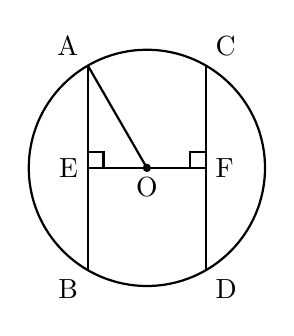
\begin{tikzpicture}[scale=1]

  % Define the center of the circle
  \coordinate (O) at (0,0);

  % Define the radius of the circle
  \def\R{1.5}

  % Draw the circle
  \draw[thick] (O) circle (\R);

  % Add a dot at the center
  \fill (O) circle (1.5pt);

  % Define points for the chords
  % AB is on the left
  \coordinate (A) at (120:\R);
  \coordinate (B) at (240:\R);
  
  % CD is on the right
  \coordinate (C) at (60:\R);
  \coordinate (D) at (300:\R);

  % Define the midpoints E and F
  % Since AB is vertical, x-coordinate is same as A and B
  \coordinate (E) at (-0.75, 0);
  % Since CD is vertical, x-coordinate is same as C and D
  \coordinate (F) at (0.75, 0);

  % Draw the chords AB and CD
  \draw[thick] (A) -- (B);
  \draw[thick] (C) -- (D);

  % Draw the line segment EF passing through center O
  \draw[thick] (E) -- (F);

  % Draw the line segment OA
  \draw[thick] (O) -- (A);

  % Draw the right-angle symbols at E and F
  \draw[thick] (-0.75,0) -- (-0.75,0.2) -- (-0.55,0.2) -- (-0.55,0);
  \draw[thick] (0.75,0) -- (0.75,0.2) -- (0.55,0.2) -- (0.55,0);

  % Add labels for the points
  \node[above left] at (A) {A};
  \node[below left] at (B) {B};
  \node[above right] at (C) {C};
  \node[below right] at (D) {D};
  \node[left] at (-0.75, 0) {E};
  \node[right] at (0.75, 0) {F};
  \node[below] at (0, 0) {O};

\end{tikzpicture}